\chapter{\IfLanguageName{dutch}{Stand van zaken}{State of the art}}%
\label{ch:stand-van-zaken}

% Tip: Begin elk hoofdstuk met een paragraaf inleiding die beschrijft hoe
% dit hoofdstuk past binnen het geheel van de bachelorproef. Geef in het
% bijzonder aan wat de link is met het vorige en volgende hoofdstuk.

% Pas na deze inleidende paragraaf komt de eerste sectiehoofding.

\begin{comment}

Dit hoofdstuk bevat je literatuurstudie. De inhoud gaat verder op de inleiding, maar zal het onderwerp van de bachelorproef *diepgaand* uitspitten. De bedoeling is dat de lezer na lezing van dit hoofdstuk helemaal op de hoogte is van de huidige stand van zaken (state-of-the-art) in het onderzoeksdomein. Iemand die niet vertrouwd is met het onderwerp, weet nu voldoende om de rest van het verhaal te kunnen volgen, zonder dat die er nog andere informatie moet over opzoeken \autocite{Pollefliet2011}.

Je verwijst bij elke bewering die je doet, vakterm die je introduceert, enz.\ naar je bronnen. In \LaTeX{} kan dat met het commando \texttt{$\backslash${textcite\{\}}} of \texttt{$\backslash${autocite\{\}}}. Als argument van het commando geef je de ``sleutel'' van een ``record'' in een bibliografische databank in het Bib\LaTeX{}-formaat (een tekstbestand). Als je expliciet naar de auteur verwijst in de zin, gebruik je \texttt{$\backslash${}textcite\{\}}.
Soms wil je de auteur niet expliciet vernoemen, dan gebruik je \texttt{$\backslash${}autocite\{\}}. In de volgende paragraaf een voorbeeld van elk.

\textcite{Knuth1998} schreef een van de standaardwerken over sorteer- en zoekalgoritmen. Experten zijn het erover eens dat cloud computing een interessante opportuniteit vormen, zowel voor gebruikers als voor dienstverleners op vlak van informatietechnologie~\autocite{Creeger2009}.

\end{comment}

In dit hoofdstuk wordt de state-of-the-art van dit onderzoek diepgaand besproken. Dit hoofdstuk biedt alle nodige informatie om de vergelijking tussen het oude en het nieuwe te vormen. Daarnaast is dit hoofdstuk de basislaag om dit onderzoek praktisch uit te werken. De titel bestaat uit drie onderdelen, namelijk: Microsoft administration, de module van Azure Active Directory en Microsoft Graph met \ac{API}. Als eerste wordt het begrip Microsoft administration besproken met bijhorende geschiedenis. Microsoft administration is de overkoepelende term waarin beide technologieën zich afspelen. Bij het tweede onderdeel wordt er dieper gekeken in dit domein. Er wordt meer duiding gegeven over Azure Active Directory met bijhorende componenten waaronder de PowerShell-module. Als laatste wordt Microsoft Graph aangeraakt met een focus op de \ac{API}. De interne werking en mogelijkheden worden hierbij gedetailleerd besproken.


\section{Wat is Microsoft administration?}

% Taalcheck OK

Microsoft administration bestaat uit twee kernwoorden die bekend zijn binnen de \ac{IT}-wereld. Microsoft staat voor het Amerikaanse technologiebedrijf en de producten die het aanbiedt \autocite{Warner2019}. Het woord administration, oftewel administratie in het Nederlands, staat voor het beheren van iets \autocite{Burgess2003}. Vanuit het woord administration volgde het woord administrator, dat duidt op een persoon die een of meerdere instanties beheert. Kortom, Microsoft administration staat voor het beheren van Microsoft-instanties en -producten (bv. Windows en Azure). 

% TODO: bv. & IT afkorting ergens noteren over zorgen dat dit hierboven komt en dan een “ac” erover maken 

\subsection{Administration in de jaren tachtig en negentig}

% Taalcheck OK

Het beheren van systemen kan omvat worden in enkele taken, hieronder volgt een lijst van frequente taken tussen het jaar 1980 en 2000 \autocite{Frisch2002}.

\begin{itemize}
    \item Toevoegen van nieuwe gebruikers en toestellen
    \item Maken en beheren van back-ups
    \item Bestanden en andere data recupereren
    \item Gebruikers assisteren in dagelijkse taken en problemen
    \item Monitoren van systemen
    \item De veiligheid van de systemen garanderen
    \item Het beheren en installeren van updates
    \item Het automatiseren van taken
\end{itemize}

Deze taken zijn vandaag de dag nog steeds herkenbaar als dagdagelijkse taken van een systeembeheerder. 

\subsection{Microsoft administration via Windows}

% Taalcheck OK

Sinds de opkomst van Windows-systemen zoals Windows 2000 server, zijn er mogelijkheden om administratieve taken uit te voeren binnen netwerkinfrastructuren \autocite{Tulloch2001}. \\

Binnen Windows 2000 server zijn er administratieve tools zoals Microsoft Management Console, Event Viewer en Active Directory Domains and Trusts-instellingen beschikbaar. Deze tools dienen om de taken van een administrator te vergemakkelijken, door een overzicht te brengen van alle data in dat specifieke onderdeel \autocite{Sibisi2022}. Door het gebruik van deze administratieve tools kan een administrator Microsoft-entiteiten waaronder Windows-toestellen beheren om zijn taken mee uit te voeren. 

\subsection{De evolutie van systemen en zijn administratie}

% Taalcheck OK

In het begin van de eenentwintigste eeuw werden systemen en servers zoals Windows 2000 server met een focus op \ac{On-prem} onderhouden \autocite{Microsoft2022a}. \ac{On-prem} betekent dat software en hardware, zoals computers en servers, op locaties staan dat eigendom is van het bedrijf en lokaal worden toegepast \autocite{Gastermann2015}. Hierbij wordt de systeemadministratie door systeembeheerders lokaal aangepakt. Ter illustratie, in dit scenario focust de automatisatie via PowerShell zich op de lokale entiteiten binnen het bedrijf. Databanken, mailservers, \ac{DNS}-servers en andere instanties worden lokaal aangesproken en geautomatiseerd indien nodig. \\

Rond het jaar 2006 evolueerde de On-premises-aanpak naar een cloud-aanpak \autocite{Hayes2008}. \ac{EC2} van Amazon is een van de grondleggers binnen de cloudservices \autocite{Qian2009}. Deze inventie van Amazon heeft sindsdien invloed op de huidige marktleiderspositie van AWS in cloud computing \autocite{Vailshery2022}. Op de tweede plaats bevindt zich de cloudservice van Microsoft, genaamd Azure.



\subsection{De impact van cloud computing op systeem administratie}

% Taalcheck OK

Cloud computing heeft een brede betekenis. Het is in feite een technologiemodel dat gebruikt wordt om middelen en diensten beschikbaar te stellen op het internet, of de cloud. \autocite{Haag2009} \\

De migratie van \ac{On-prem} naar de cloud is geen toeval. Eenenveertig procent van de bedrijven uit de \ac{EU} maakt gebruik van cloud computing in 2021 \autocite{EU2021}. \\

Het gebruik van cloud computing en cloudservices heeft vele voordelen. De volgende lijst bevat enkele voordelen van cloud computing. De lijst is samengesteld uit onderzoek van \textcite{Aljabre2012}, \textcite{Rittinghouse2016}.

\begin{itemize}
    \item Minder onderhouds-, implementatie- en infrastructuurkosten.
    \item Goedkopere computers per gebruiker (via virtuele machines).
    \item Verhoogde mobiliteitskansen voor de werkkrachten.
    \item Nieuwe en flexibelere infrastructuren met verhoogde schaalbaarheid.
    \item Vergroening van data centers.
    \item Verhoogde beschikbaarheid van applicaties.
    \item Mogelijkheid om gebruikers te doen samenwerken in documenten en projecten.
\end{itemize}



\subsection{Verschuiving van On-premises naar de cloud}

% Taalcheck

De evolutie van \ac{On-prem} naar de cloud heeft invloed op de huidige stand van zaken binnen Microsoft administration. Microsoft administratie staat in voor het beheren van Microsoft-entiteiten. Door een verschuiving van \ac{On-prem} naar cloudomgevingen, wordt de nadruk stilaan gelegd op het beheren van bepaalde entiteiten via cloudtoepassingen. \\

Deze nadruk valt op wanneer de productenlijst van Microsoft Azure wordt geraadpleegd \autocite{Microsoft2023b}. Dit is een lijst die steeds verder wordt uitgebreid met nieuwe technologieën. \\

Een praktisch voorbeeld van een entiteit, of een groep van entiteiten, dat via de cloud kan beheerd worden is Azure Active Directory \autocite{Microsoft2023c}. Azure Active Directory kan gebruikt worden als alternatief voor Active Directory voor bepaalde onderdelen. Active Directory is kortweg een opslagplaats die een focus heeft op On-premises-instanties. Active Directory en Azure Active Directory worden in het volgende onderdeel verder besproken.

% ---
% Volgende onderdeel
% ---

\section{Wat is Azure Active Directory?}

\ac{AD} is een centrale en gemeenschappelijke opslagplaats voor informatie geïntroduceerd door Microsoft \autocite{Allen2003}. De eerste versie van \ac{AD} is gemaakt voor de Windows 2000 server-editie. Deze opslagplaats bevat allerlei informatie binnen een netwerk, zoals gebruikers, groepen, computers, applicaties, bestanden en printers. Deze informatie kan worden opgevraagd en beheerd. \\

Azure \ac{AD} is een modernere aanpak van Active Directory binnen de cloud dat ontstaan is in 2008 \autocite{Chappell2008}. Azure \ac{AD} is een gecentraliseerd beheerplatform van Microsoft voor gebruikers en apparaten in netwerken die een verbinding hebben met de Azure-clouddienst \autocite{Mayank2019}. Middelen, waaronder gebruikers en apparaten, kunnen vanuit Azure \ac{AD} beheerd worden met bijhorende netwerkauthenticatie. Het dient als een centraal punt van informatie, waarbij details over alle middelen in het netwerk worden opgeslagen.

\subsection{Azure Active Directory PowerShell-modules} 

Azure \ac{AD} PowerShell voor Graph, kortweg Azure \ac{AD} PowerShell, is een module binnen PowerShell die gebruikt kan worden om Azure \ac{AD} te beheren \autocite{Microsoft2023}. PowerShell is een oplossing van Microsoft voor taakautomatisering via een \ac{CLI} \autocite{Microsoft2022}. \\

PowerShell staat gekend voor zijn breed scala aan informatie dat het kan verkrijgen. Dit breed scala gaat van systemen, servers, randapparatuur, mobiele apparaten tot gegevensgestuurde toepassingen zoals Active Directory \autocite{Hosmer2019}. Vandaag de dag ondersteunt PowerShell meer dan 11.350 unieke modules en scripts via de PowerShell Gallary, waaronder de Azure \ac{AD} PowerShell module \autocite{Microsoft2023a}. \\

Door het gebruik van Azure \ac{AD} in combinatie met PowerShell, wordt er gebruikgemaakt van het beste van de twee werelden. Een gecentraliseerd beheerplatform automatisch doen werken brengt bijkomende voordelen voor de maker. Uit onderzoek van \textcite{Breton2003} zijn enkele voordelen van automatisatie minder stress, tijdbesparing en een lagere kans op menselijke fouten. \\

Naast de Azure \ac{AD} PowerShell-module, is er de MSOnline PowerShell-module \autocite{Prigent2019}. MSOnline is de voorganger van de AzureAD-module. MSOnline is de eerste versie, in vergelijking met AzureAD dat de tweede versie is. MSOnline heeft dezelfde functie als AzureAD en biedt de mogelijkheid aan om via PowerShell Azure \ac{AD} te kunnen aanspreken.

\subsubsection{Ondersteunende data-objecten}

PowerShell heeft verschillende soorten commando's voor het toevoegen, verwijderen of lezen van iets. Wanneer een commando de functie heeft om iets op te vragen, dan kan dit bijvoorbeeld een “Get”-commando zijn zoals “Get-MgUser”. \\

Binnen Azure AD PowerShell zijn er twaalf soorten commando's, namelijk:

\begin{itemize}
    \item Add: Toevoegen.
    \item Confirm: Bevestigen.
    \item Connect: Verbinden.
    \item Disconnect: Ontkoppelen.
    \item Get: Informatie ophalen.
    \item New: Aanmaken.
    \item Remove: Verwijderen.
    \item Restore: Herstellen.
    \item Revoke: Intrekken.
    \item Select: Informatie ophalen.
    \item Set: Wijzigen.
    \item Update: Bijwerken.
\end{itemize}

Azure AD PowerShell ondersteunt volgende data-objecten met een specifiek aantal uitvoerbare commando's \autocite{Microsoft2023i}. Per data-object zijn er een of meerdere soorten PowerShell-commando's, in de tabel wordt alleen het aantal commando's weergegeven. Een overzicht van alle ondersteunde data-objecten met het aantal commando's wordt weergeven in Tabel \ref{AADT}. 

\begin{table}
    \small
    \centering
    \begin{tabular}{ |c|c| } 
        \hline
        \textbf{Data-object} & \textbf{Aantal commando's} \\
        \hline
        Administrative Units & 9 \\ 
        Application Proxy Application Management & 8 \\ 
        Application Proxy Connector Management & 9 \\
        Applications & 20 \\ 
        AzureAD & 49 \\ 
        Certificate Authorities & 4 \\ 
        Connect to directory & 2 \\ 
        Contacts & 8 \\ 
        Contracts & 1 \\ 
        Deleted Objects & 1 \\ 
        Devices & 11 \\    
        Directory & 3 \\
        Directory Objects & 1 \\ 
        Directory Roles & 13 \\ 
        Domains & 8 \\ 
        Extension Properties & 1 \\ 
        Groups & 26 \\ 
        MSOnline & 97 \\
        OAuth2 & 2 \\ 
        Policies & 2 \\ 
        Service Principals & 22 \\ 
        Users & 30 \\ 
        \hline
    \end{tabular}
    \caption[Tabel Azure AD en MSonline data-objecten]{Tabel met overzicht van alle ondersteunende data-objecten van Azure \ac{AD} en MSOnline met bijhorende commando's binnen Azure \ac{AD} PowerShell.}
    \label{AADT}
\end{table}

\subsection{Wat is Azure Active Directory Graph?}

% TODO: uitleggen wat MSOnline is ??? (niet hier maar ergens anders)

De communicatie tussen Azure \ac{AD} en de Azure \ac{AD} PowerShell-module gebeurd via een \ac{API}. Deze \ac{API} is een \ac{REST} \ac{API} die Graph wordt genoemd. \\ 

De naam Graph is afgeleid uit het wiskundige figuur van een graaf. Een graaf is een verzameling van punten die wel of niet met elkaar zijn verbonden \autocite{Denaux2022}. Een voorbeeld van een wiskundige graaf is te zien op Figuur \ref{mga}. \\

\begin{figure}[!b]
    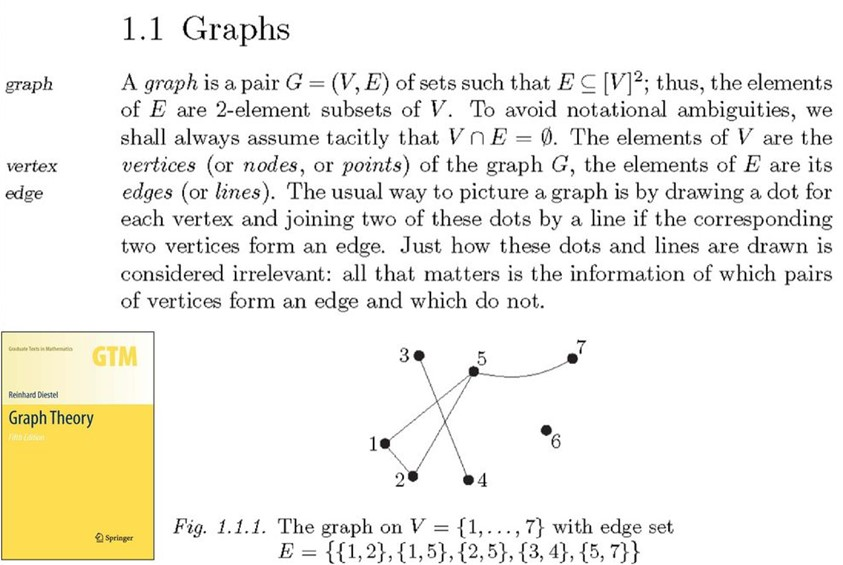
\includegraphics[width=\textwidth]{MathGraphExample.jpg}
    \caption[Voorbeeld wiskundige graaf]{Voorbeeld van een graaf in de wiskunde uit het boek Graph Theory van \textcite{Diestel2010}.}
    \label{mga}
\end{figure}

Graph van Microsoft heeft een soortgelijke betekenis als dat van een wiskundige graaf. Graph staat in voor de verbindingen tussen de entiteiten dat het ondersteunt, in dit geval Microsoft-entiteiten \autocite{Kokkarinen2022}. Een logische interpretatie van Graph wordt weergegeven op Figuur \ref{gms}. \\

\begin{figure}[!b]
    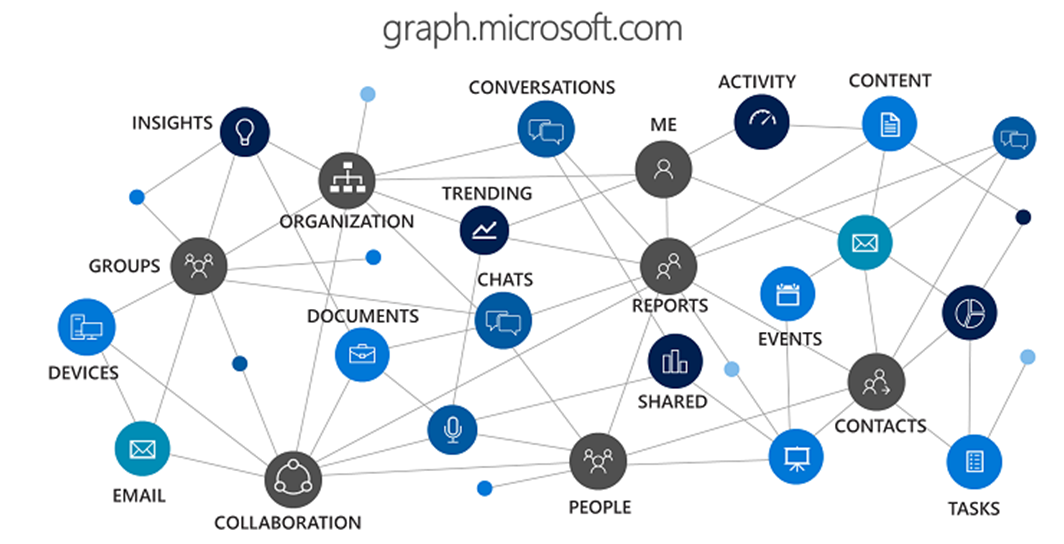
\includegraphics[width=\textwidth]{GraphMicrosoft.png}
    \caption[Voorbeeld Azure AD Graph]{Voorstelling van Azure \Ac{AD} Graph door \textcite{Microsoft2017}.}
    \label{gms}
\end{figure}

\subsubsection{Achterliggende werking van Azure Active Directory Graph API}

% TODO: Bronnen (zie word onder Azure AD Graph API)

% TODO: Schrijf verder vanuit de bron van weareminky, dit is de makkelijkste manier

De Azure \ac{AD} Graph \ac{API} is een OData 3.0-compatibele dienst om objecten zoals gebruikers, groepen en contactpersonen in een tenant te lezen en te wijzigen \autocite{Microsoft2016}. \\

Een tenant kan vergeleken worden met een appartementencomplex \autocite{Saxton2015}. Binnen dit complex zijn meerdere appartementen. In elk appartement heb je bijvoorbeeld een badkamer, slaapkamer, living en balkon. Deze uitleg wordt gevisualiseerd op Figuur \ref{rlt}. \\

\begin{figure}[!h]
    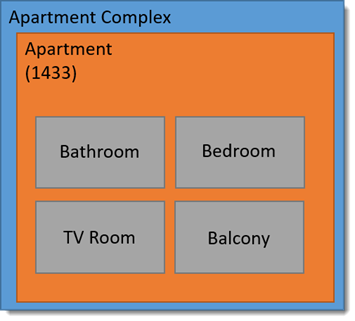
\includegraphics[width=50mm, scale=0.5]{RealTenant.png}
    \caption[Voorbeeld werkelijke tenant]{Voorbeeld van een tenant in het echte leven uit de blog van \textcite{Saxton2015}.}
    \label{rlt}
\end{figure}

In dit scenario met Microsoft is (in \ac{IT}-termen) het complex de Microsoft Office 365-datacenters. Het appartement stelt de tenant of de organisatie in het algemeen voor. Deze tenant-omgeving bevat bijvoorbeeld abonnementen, gebruikers, domeinen en groepen. De tenant wordt gezien als een huurder van de omgeving. Dit concept wordt gevisualiseerd op Figuur \ref{mst}. \\

\begin{figure}[!h]
    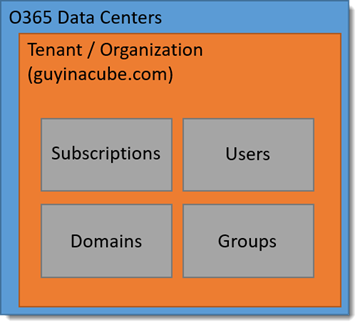
\includegraphics[width=50mm, scale=0.5]{MSTenant.png}
    \caption[Voorbeeld Microsoft tenant]{Voorbeeld van een tenant binnen Microsoft uit de blog van \textcite{Saxton2015}.}
    \label{mst}
\end{figure}

Het OData-protocol dient voor interacties met gegevens via \ac{REST}-webdiensten. Dit protocol biedt een uniforme manier om gegevens en gegevensmodellen te beschrijven \autocite{OData2023}. \\

Door het gebruik van \ac{REST}-eindpunten kunnen \ac{HTTP}-verzoeken verstuurd worden om bewerkingen uit te voeren met de service. De Azure \ac{AD} Graph \ac{API} heeft een eigen demo-omgeving genaamd Azure \ac{AD} Graph Explorer, waarin bepaalde functies en bewerkingen worden getest \autocite{Microsoft}. \\

Het proces van Graph gaat van start wanneer een applicatie een verzoek doet. Dit verzoek moet een token bevatten. Deze token wordt gegeven door Azure \ac{AD} en bewijst dat de gebruiker de juiste machtigingen heeft om de gevraagde data te raadplegen.



\subsubsection{Authenticatie via libraries}

Vooraleer de autorisatie kan plaatsvinden, moet er eerst worden geauthenticeerd. Dit gebeurd via een tool genaamd \ac{ADAL} of de modernere \ac{MSAL} van \textcite{Microsoft2022d}. \\

\ac{ADAL} en \ac{MSAL} worden gebruikt voor verificatie- en autorisatiefunctionaliteiten \autocite{Ooms2022}. Beide technologieën dienen om te kunnen authenticeren met de Graph \ac{API}. \\ 

Er zijn twee methodes om te verbinden met de Graph \ac{API}. \\

De eerste is door middel van een gedelegeerde of interactieve manier. Er wordt gebruikgemaakt van een prompt waarbij de gebruikersnaam (of mailadres) en het wachtwoord wordt gevraagd. \\

Bovendien kan er gevraagd worden om een \ac{2FA}- of \ac{MFA}-methode toe te passen. Dit gaat gepaard met het account waarop de gebruiker wilt inloggen, indien dit geactiveerd is. \\

Het gebruik van \ac{2FA} of \ac{MFA} is veiliger dan alleen het gebruik van een naam en wachtwoord, bevestigt het onderzoek van \textcite{Gunson2011} en \textcite{Banyal2013}. Het wordt sterk aangeraden om minstens \ac{2FA} toe te passen bij het gebruik van een gedelegeerde methode. \\

De tweede methode is door een niet-interactieve of geprogrammeerde manier. Deze methode maakt gebruik van secrets die aan de registratie van een applicatie is gekoppeld. Deze registratie gebeurd in Azure. 



\subsubsection{Autorisatie door middel van tokens}

Azure Active Directory-tokens bevatten informatie over de applicatie, de gebruiker, authenticatie en de rechten die een applicatie mag uitvoeren op de bijhorende directory \autocite{Microsoft2015}. \\

Deze tokens bevinden zich in de autorisatieheader van een verzoek.
Een afgekort voorbeeld hiervan is te zien op Figuur \ref{ahtoken}. \\

\begin{figure}[h]
    \begin{verbatim}Authorization: Bearer eyJ0eX ... FWSXfwtQ
    \end{verbatim}    
    \caption[Voorbeeld Azure AD-token]{Afgekort voorbeeld van een Azure \Ac{AD}-token binnen een autorisatieheader.}
    \label{ahtoken}
\end{figure}

Vervolgens voert de \ac{API} de nodige autorisaties uit via permissie scopes. Dit zijn OAuth 2.0 permissie scopes die aanwezig zijn in het Azure \Ac{AD}-token. OAuth 2.0 is een standaardprotocol voor autorisatie \autocite{OAuth}. \\

De permissie scopes worden gebruikt om te controleren of een gebruiker toegang heeft tot een bepaalde map of locatie. Een ontwikkelaar moet in dit scenario de juiste permissie scopes gebruiken om over de vereiste rechten te beschikken voor een actie. \\

Wanneer er wordt aangemeld, krijgt de gebruiker de mogelijkheid om toestemming te geven of de applicatie in kwestie de mapgegevens van de gebruiker mag benutten. Tijdens het toestaan worden de permissie scopes meegegeven die de ontwikkelaar heeft ingesteld. Een opsomming van de mogelijk permissie scopes binnen de Azure \ac{AD} Graph \ac{API} bevindt zich in Tabel \ref{psaad}. 

\begin{table}
    \footnotesize
    \centering
    \begin{tabular}{ |c|c| } 
        \hline
        \textbf{Scope} & \textbf{Beschrijving} \\
        \hline
        User.Read & Rechten om aan te melden en het gebruikersprofiel te lezen. \\
        User.ReadBasic.All & Rechten om de basisprofielen van alle gebruikers te lezen. \\
        User.Read.All & Rechten om het volledige profiel van alle gebruikers te lezen. \\
        Group.Read.All & Rechten om alle groepen te lezen. \\
        Group.ReadWrite.All & Rechten om alle groepen te lezen en te bewerken. \\
        Device.ReadWrite.All & Rechten om alle apparaten te lezen en te bewerken. \\
        Directory.Read.All & Rechten om alle mapgegevens te lezen. \\
        Directory.ReadWrite.All & Rechten om alle mapgegevens te lezen en te bewerken. \\
        Directory.AccessAsUser.All & Rechten om in de map toe treden als de aangemelde gebruiker. \\
        \hline
    \end{tabular}
    \caption[Tabel Azure \ac{AD} Graph Permission scopes]{Tabel met de beschikbare permissie scopes bijhorende beschrijving door \textcite{Microsoft2016a}.}
    \label{psaad}
\end{table}

Het gebruik van permissie scopes komt overeen met een gekend veiligheidsprincipe binnen de \ac{IT}. “Principle of Least Privilege”, of “Beginsel van de minste voorrechten” in het Nederlands, staat voor het toekennen van een minimum aan rechten \autocite{Saltzer1975}. 



\subsubsection{Eindpunt adressering}

Om taken of functies uit te voeren met de Graph \ac{API}, wordt er gebruikgemaakt van \ac{HTTP}-verzoeken. Deze verzoeken maken gebruik van een bepaalde methode. Een opsomming van de mogelijk methodes wordt hieronder weergegeven met bijhorende betekenis, gebaseerd op het onderzoek van \textcite{Fielding1999}, \textcite{Dusseault2010}.

\begin{itemize}
    \item GET: Geeft data weer van de server.
    \item POST: Verstuurt data naar de server om nieuwe data aan te maken.
    \item PATCH: Verstuurt data naar de server om gedeeltelijk de bron bij te werken.
    \item PUT: Verstuurt data naar de server om de volledige bron bij te werken.
    \item DELETE: Verwijdert data van de server.
\end{itemize}

Deze verzoeken zijn gericht op een eindpunt van een dienst, een resource, een verzameling van resources of andere entiteiten die de \ac{API} ondersteunt. De eindpunten worden genoteerd als een \ac{URL}. Het gebruikelijk formaat van zo'n eindpunt wordt voorgesteld op Figuur \ref{bfe}. \\

\begin{figure}[h]
    \footnotesize\begin{verbatim}https://graph.windows.net/{tenant_id}/{resource}?{version}&query-parameters
    \end{verbatim}    
    \caption[Basis formaat Graph API-eindpunt]{Het basis formaat van een Azure \ac{AD} Graph \ac{API}-eindpunt uit documentatie van \textcite{Microsoft2023o}.}
    \label{bfe}
\end{figure}

De reeds voorgestelde \ac{URL} bestaat uit vier componenten.

\begin{itemize}
    \item Service root: Het aanspreekpunt voor alle Graph \ac{API}-verzoeken. Voor Azure \ac{AD} Graph is dit “https://graph.windows.net”.
    \item Tenant Identifier: De identiteit van de tenant waar het verzoek naar gericht is.
    \item Resource path: Het pad van de bron waar het verzoek naar gericht is.
    \item Graph \ac{API} version: De versie van de \ac{API} waar het verzoek naar gericht is.
\end{itemize}

Een praktisch voorbeeld met betrekking tot het oproepen van gebruikersgegevens, wordt weergegeven op Figuur \ref{pfe}. \\

\begin{figure}[h]
    \footnotesize\begin{verbatim}https://graph.windows.net/contoso.com/users/john@contoso.com/
$links/manager?api-version=1.6
    \end{verbatim}    
    \caption[Voorbeeld Graph API-eindpunt]{Praktisch voorbeeld van een Graph \ac{API}-eindpunt, gericht op de manager eigenschap van “john@contoso.com”.}
    \label{pfe}
\end{figure}



\subsubsection{OData Query Parameters}

Zoals reeds vermeld maakt de Graph \ac{API} gebruik van OData. Het gebruik van OData-queryparameters zorgt ervoor dat een ingelezen verzameling van bronnen kunnen gefilterd, gesorteerd en gepagineerd worden. \\

De Graph \ac{API} biedt ondersteuning aan voor de volgende parameters met bijhorende betekenis. De betekenissen staan gedefinieerd in studies van \textcite{Liang2016}, \textcite{Wojcieszyn2014}. 

\begin{itemize}
    \item \$batch: Indienen van \ac{HTTP} POST-verzoeken.
    \item \$expand: Opnemen van een of meerdere bronnen in het antwoord.
    \item \$filter: Filteren van beschikbare bronnen.
    \item \$orderby: Opgeven van ordening door de opgevraagde collectie.
    \item \$previous-page: Ophalen van vorige pagina met resultaten.
    \item \$top: Beperken van een teruggezonden opgevraagde verzameling.
    \item \$skiptoken: Overslaan van opgegeven aantal items.
\end{itemize}

Een toegepast voorbeeld van een OData-queryparameter is te vinden in Figuur \ref{odqp}. \\

\begin{figure}[h]
\footnotesize\begin{verbatim}GET https://graph.windows.net/contoso.com/directoryObjects?api-version=2013-04-05&
$filter=isof('Microsoft.WindowsAzure.ActiveDirectory.User')%20or%20isof
('Microsoft.WindowsAzure.ActiveDirectory.Group')%20or%20isof
('Microsoft.WindowsAzure.ActiveDirectory.Contact')&deltaLink=HTTP/1.1
\end{verbatim}    
\caption[Voorbeeld OData-queryparamter]{Toegepast voorbeeld van een OData-queryparameter op een \ac{HTTP} GET-request.}
\label{odqp}
\end{figure}

\subsubsection{Request en Response Headers}

% TODO: Bron zoeken voor onderstaande uitleg?

De Graph \ac{API} werkt met verzoeken en antwoorden. Een verzoek werkt met een aantal soorten headers en bodies. \\

Drie voorbeelden van voorkomende verzoekheaders zijn de volgende:

\begin{itemize}
    \item Authorization: Uitgegeven Azure \ac{AD}-token.
    \item Content-Type: Mediatype van de inhoud.
    \item Content-Length: Lengte van het verzoek (in bytes).
\end{itemize} 

Daarnaast bestaan er ook een aantal antwoordheaders. Hieronder worden een aantal mogelijke antwoordheaders meegegeven met hun betekenis.

\begin{itemize}
    \item Content-Type: Mediatype van de inhoud.
    \item Location: Antwoord op POST-verzoeken wanneer een nieuwe bron in de directory wordt aangemaakt.
    \item ocp-aad-diagnostics-server-name: Identifier voor de server die een bewerking uitvoert.
    \item ocp-aad-session-key: Sleutel die een sessie met de directorydienst identificeert.
\end{itemize}

Een voorbeeld van antwoordheaders binnen Azure \ac{AD} Graph wordt weergegeven bij Listing \ref{rhaad}. \\

\begin{listing}[h]
\begin{minted}
[
frame=lines,
framesep=2mm,
baselinestretch=1.2,
fontsize=\footnotesize,
linenos
]  
{json}
{
    "cache-control": "no-cache",
    "client-request-id": "140987df-c416-44b8-bf96-16d550256bad",
    "content-length": "12478",
    "content-type": 
        "application/json; 
        odata=minimalmetadata; 
        streaming=true; 
        charset=utf-8",
    "expires": "-1",
    "ocp-aad-session-key": "MzsMU-KCo5fDEUHgzYfj ... hf8ZctaauwL-EZo",
    "pragma": "no-cache",
    "request-id": "c7f02989-6a03-444a-abb2-e3c7993c1ded"
}
    \end{minted}
    \caption[Voorbeeld Response Headers Azure AD Graph]{Voorbeeld van Response Headers binnen Azure \ac{AD} Graph via Azure \Ac{AD} Graph Explorer.}
    \label{rhaad}
\end{listing}

\subsubsection{Request en Response Bodies}

Request bodies kunnen via \Ac{JSON}- of \ac{XML}-payloads verzonden worden voor POST-, PATCH- en PUT-verzoeken. Bovendien kunnen antwoorden (van een server) worden teruggestuurd via \ac{JSON} of \ac{XML}. \\

Het woord “payload” staat voor data die via een pakket of transmissie worden gedragen \autocite{Comer2006}. \\

Deze payloads kunnen in de request bodies gespecifieerd worden via de Content-Type verzoekheader en in antwoorden van Accept-verzoekheaders. \\

Een voorbeeld van een request, met bijhorende request en response body, wordt voorgesteld bij Listing \ref{hpr}, \ref{hreqb} en \ref{hresb}. \\

\begin{listing}[h]
\begin{verbatim}
POST https://graph.windows.net/myorganization/users?api-version
\end{verbatim}
\caption[Voorbeeld HTTP POST-request]{Voorbeeld van een \ac{HTTP} POST-request binnen Azure \ac{AD} Graph.}
\label{hpr}
\end{listing}

\begin{listing}[!b]
\begin{minted}
[
frame=lines,
framesep=2mm,
baselinestretch=1.2,
fontsize=\footnotesize,
linenos
]  
{json}
{
    "accountEnabled": true,
    "displayName": "Alex Wu",
    "mailNickname": "AlexW",
    "passwordProfile": {
        "password": "Test1234",
        "forceChangePasswordNextLogin": false
    },
    "userPrincipalName": "Alex@a830edad9050849NDA1.onmicrosoft.com"
}
\end{minted}
\caption[Voorbeeld Request Body Azure AD Graph]{Voorbeeld van een Request Body binnen Azure \ac{AD} Graph.}
\label{hreqb}
\end{listing}

\begin{listing}[!t]
\begin{minted}
[
frame=lines,
framesep=2mm,
baselinestretch=1.2,
fontsize=\footnotesize,
linenos
]  
{json}
{
    "odata.metadata": "https://graph.windows.net/myorganization\n
    /$metadata#directoryObjects/Microsoft.DirectoryServices.User/@Element",
    "odata.type": "Microsoft.DirectoryServices.User",
    "objectType": "User",
    "objectId": "84fba1e8-b942-47c9-a10e-a4bee353ce60",
    "deletionTimestamp": null,
    "accountEnabled": true,
    "assignedLicenses": [],
    "assignedPlans": [],
    "city": null,
    "country": null,
    "department": null,
    "dirSyncEnabled": null,
    "displayName": "Alex Wu",
    "facsimileTelephoneNumber": null,
    "givenName": null,
    "immutableId": null,
    "jobTitle": null,
    "lastDirSyncTime": null,
    "mail": null,
    "mailNickname": "AlexW",
    "mobile": null,
    "onPremisesSecurityIdentifier": null,
    "otherMails": [],
    "passwordPolicies": null,
    "passwordProfile": null,
    "physicalDeliveryOfficeName": null,
    "postalCode": null,
    "preferredLanguage": null,
    "provisionedPlans": [],
    "provisioningErrors": [],
    "proxyAddresses": [],
    "sipProxyAddress": null,
    "state": null,
    "streetAddress": null,
    "surname": null,
    "telephoneNumber": null,
    "usageLocation": null,
    "userPrincipalName": "alex@a830edad9050849NDA1.com",
    "userType": "Member"
}
\end{minted}
\caption[Voorbeeld Response Body Azure AD Graph]{Voorbeeld van een Response Body binnen Azure \ac{AD} Graph.}
\label{hresb}
\end{listing}

% ---
% Volgend onderdeel
% ---

\section{Wat is Microsoft Graph?}

Microsoft Graph is, net zoals de reeds besproken Azure \Ac{AD} Graph, een centrale \ac{REST} \ac{API} voor Microsoft-entiteiten. Deze technologie is verschillend, maar volgt de uitfaserende Azure \ac{AD} Graph op \autocite{Microsoft2023n}. Microsoft Graph werd door \textcite{Microsoft2015a} in de schijnwerper gezet in 2015. \\

De technologie is gebasseerd op de wiskundige graaf, zoals ook reeds besproken werd bij Azure \Ac{AD} Graph. Microsoft Graph integreert applicaties met verschillende programmeertalen en platformen. Het logisch concept van Graph wordt weergegeven op Figuur \ref{msg}.

\begin{figure}[h]
    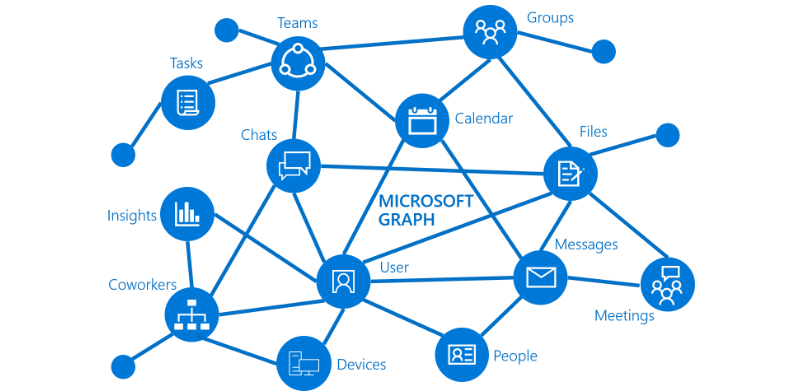
\includegraphics[width=\textwidth]{MicrosoftGraph.png}
    \caption[Voorbeeld Microsoft Graph]{Voorstelling van Microsoft Graph door \textcite{Microsoft2023d}.}
    \label{msg}
\end{figure}

\subsection{Uitfasering van Azure AD Graph}
 
Microsoft Graph bepaalde PowerShell-modules die de Azure \ac{AD} en MSOnline PowerShell-modules kunnen vervangen. Op 30 september 2022 maakte Microsoft bekend dat de uitfasering van de Azure \ac{AD} PowerShell-modules en \ac{ADAL} van start zou gaan op 30 juni 2023 \autocite{Sahay2022}. \\

De reden waarom Microsoft deze overgang in gang zet, ontstaat uit volgende redenen volgens \textcite{Microsoft2023e}:

\begin{itemize}
    \item Het gebruik van Microsoft Graph ligt dubbel zo hoog dan dat van Azure \ac{AD} Graph.
    \item Microsoft Graph bevat meer dan 150 nieuwe functies.
    \item Microsoft Graph biedt meer veiligheid en is veerkrachtiger.
    \item Microsoft Graph client libraries bevatten een ingebouwde ondersteuning voor bepaalde functies, waaronder
    \begin{itemize}
        \item herhaalde verwerkingshandelingen,
        \item veilige doorverwijzing,
        \item transparante verificatie,
        \item en payloadcompressie.
    \end{itemize}
    \item Verbeterde mogelijkheden zoals Microsoft 365-groepsbeheer, uitnodiging voor externe gebruikers en anderen.
\end{itemize} 

\subsubsection{Uitfasering van ADAL}

Naast de uitfasering van de Azure \ac{AD} PowerShell-modules, start ook de uitval van \ac{ADAL} op 30 juni 2023. Zoals reeds besproken in Azure \ac{AD} wordt er gebruikgemaakt van \ac{ADAL} of \ac{MSAL} om met de oude als nieuwe Graph te kunnen verbinden. \\

De migratie naar \ac{MSAL} brengt voordelen met zich mee, dat \ac{ADAL} niet kan aanbieden, verklaard \autocite{Microsoft2023m}. Daarnaast is \ac{MSAL} gebouwd om met het Microsoft identity platform te werken, dat de werking met Microsoft Graph vereenvoudigd.



\subsection{Microsoft Graph toepassingen}

Microsoft Graph bestaat uit drie toepassingen. \\

De eerste toepassing is de Microsoft Graph \Ac{API}. Dit is een eindpunt dat kan aangesproken worden via “https://graph.microsoft.com” dat Microsoft-entiteiten binnen de cloud kan aanspreken. Dit onderdeel wordt later dieper besproken. \\

De tweede toepassing is Microsoft Graph connectors. Deze Graph-connectoren werken in de ingaande richting. Door het gebruik van deze connectoren, kunnen gegevens buiten de Microsoft-cloud worden gestuurd naar Graph en bijhorende toepassingen. \\

Door het gebruik van deze connectors vermindert de overhead, doordat de informatie bereikbaar is. Deze bereikbaarheid is te danken aan het gebruik van eindpunten zoals SharePoint, Office.com of Bing.com dat de connectors ondersteunen. Op Figuur \ref{MSGC} wordt de werking van Connectors geïllustreerd. \\

\begin{figure}[!h]
    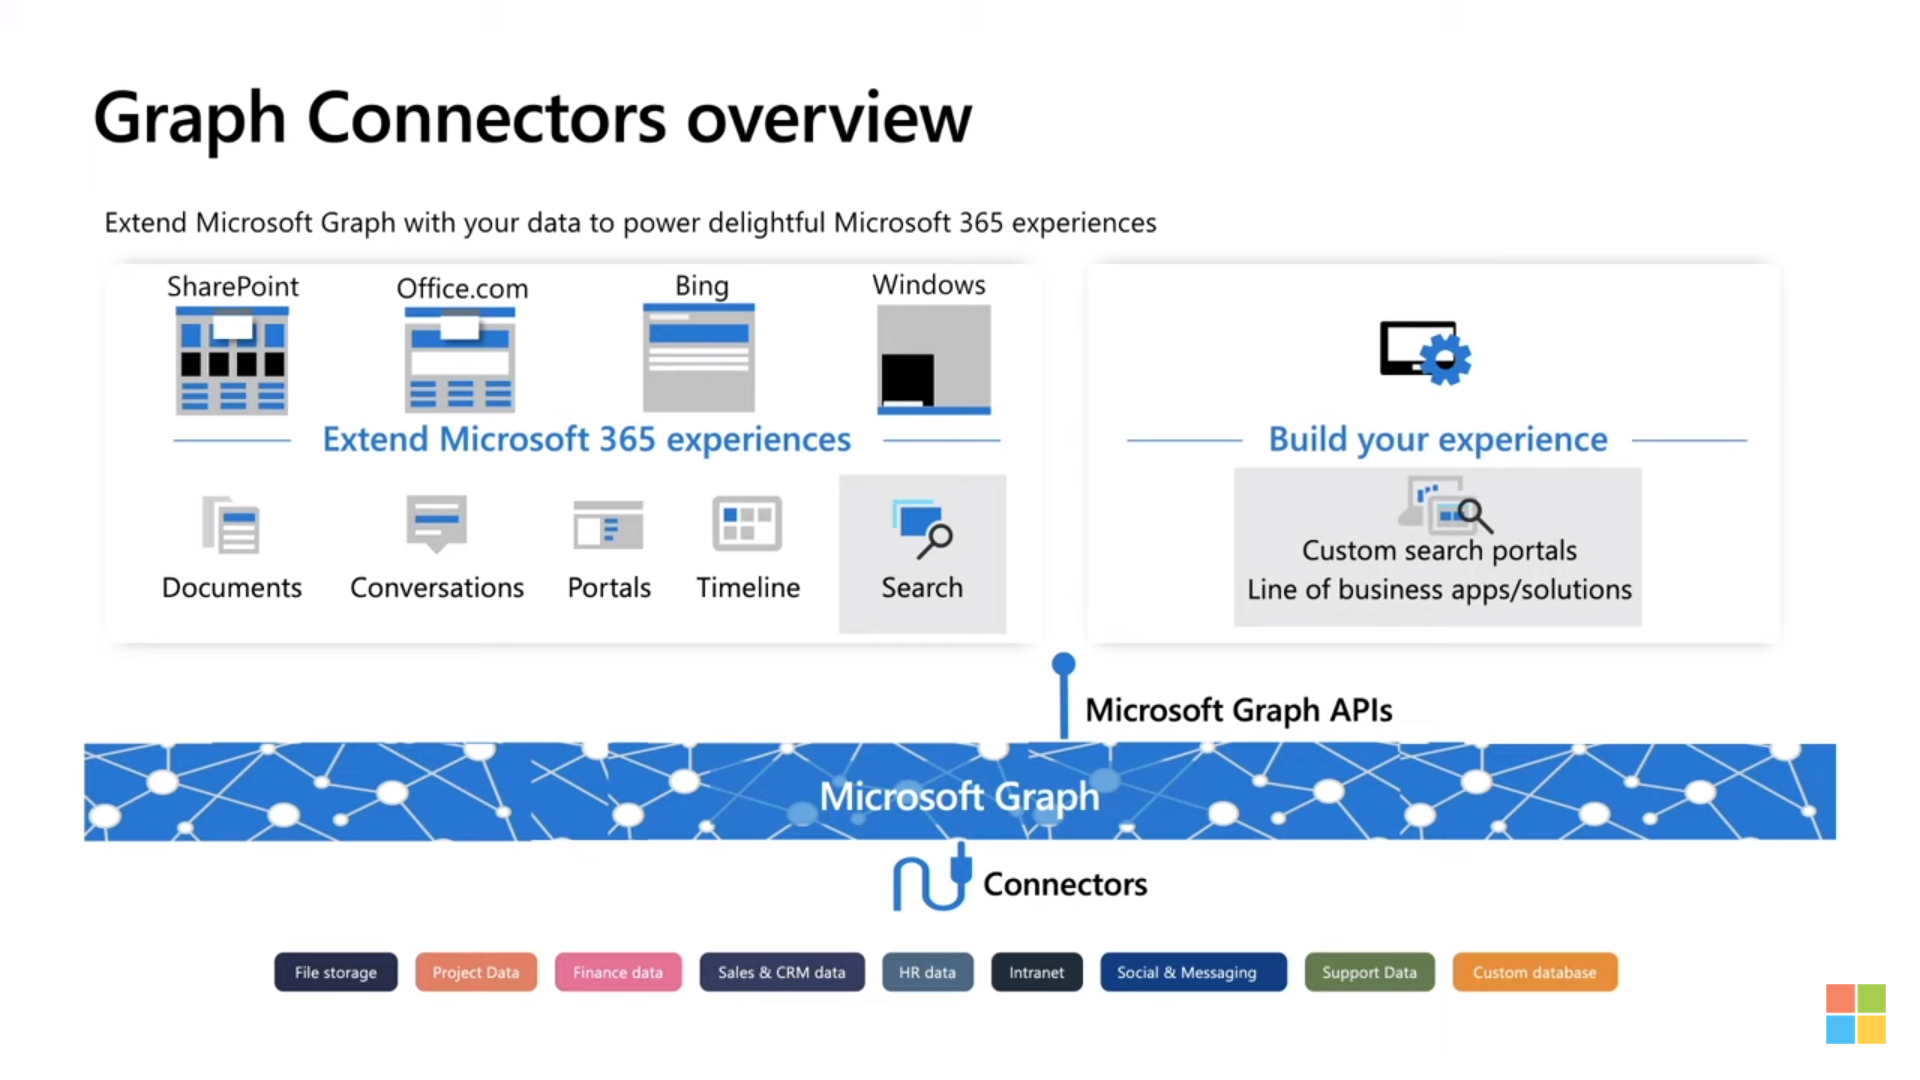
\includegraphics[width=\textwidth]{GraphConnectors.png}
    \caption[Voorbeeld Microsoft Graph Connectors]{Voorstelling van Connectors binnen Microsoft Graph door \textcite{Hay2021}.}
    \label{MSGC}
\end{figure}

Als laatste worden er een set van tools aangeboden via Microsoft Graph Data Connect. Deze tools kunnen gebruikt worden om applicaties te ontwikkelen voor analyse, intelligentie en bedrijfsprocesoptimalisatie met Microsoft 365-data. Deze data wordt geïntegreerd binnen Azure, zodat de reken- en opslagcapaciteiten van het cloudplatform worden gebruikt. Een voorstelling van Data Connect is te zien op Figuur \ref{MSGDC}. \\

\begin{figure}[!h]
    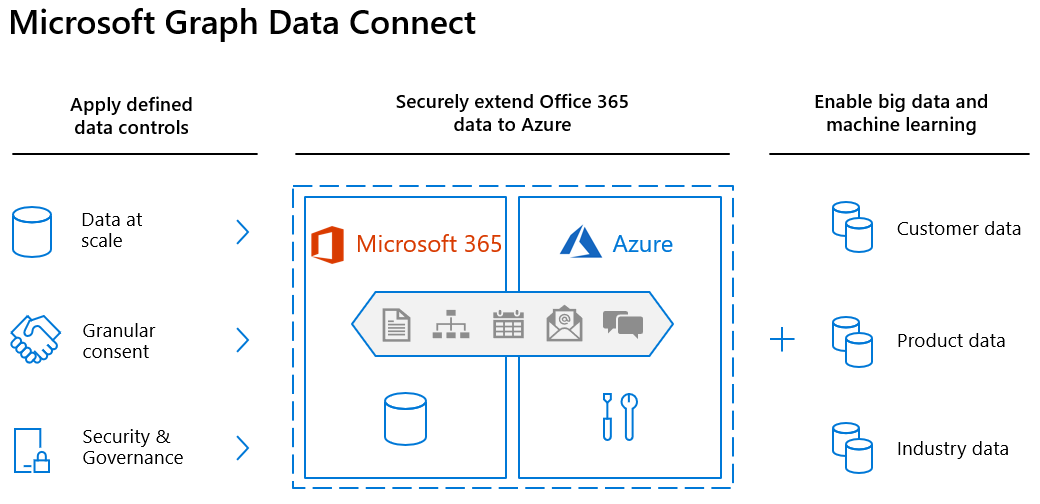
\includegraphics[width=\textwidth]{GraphDataConnect.png}
    \caption[Voorbeeld Microsoft Graph Data Connect]{Voorstelling van Data Connect binnen Microsoft Graph door \textcite{Microsoft2022c}.}
    \label{MSGDC}
\end{figure}

\subsection{Authenticatie en Autorisatie}

Vooraleer er een token wordt uitgegeven, moet een applicatie geregistreerd zijn in het Microsoft identity platform \autocite{Microsoft2022b}. Bovendien moet de applicatie beschikken over de juiste machtigingen om Microsoft Graph te mogen gebruiken. \\

\subsubsection{Toegangsmogelijkheden}

Binnen Microsoft Graph zijn er twee mogelijkheden om toegang te verschaffen tot de gegevens. Dit kan via de gedelegeerde- of App-only-methode. Een simpele weergave van wat deze methodes betekenen wordt weergegeven op Figuur \ref{MIPM}. \\

\begin{figure}[h]
    \includegraphics[width=\textwidth]{MIPmethods.png}
    \caption[Voorbeeld toegangsmogelijkheden]{Voorstelling van de twee mogelijke methodes om toegang te krijgen tot het Microsoft identity platform door \autocite{Microsoft2022b}.}
    \label{MIPM}
\end{figure}

De eerste methode, delegated access, staat voor het toegang hebben namens de gebruiker. Dit is mogelijk wanneer een gebruiker zich aanmeldt bij een applicatie. Hierdoor geeft de gebruiker toestemming. Vervolgens kan Microsoft Graph in naam van de gebruiker een actie uitvoeren. Zowel de applicatie als de gebruiker moet over de juiste machtigingen beschikken om het verzoek te laten doorgaan. \\

Een ander woord voor gedelegeerde machtigingen zijn scopes. Deze scopes maken gebruik van OAuth2-permissies. Dit concept werd al reeds besproken bij Azure \ac{AD} Graph. \\

App-only access is de tweede methode. Dit principe werkt zonder een gebruiker om met gegevens te interageren. Dit principe komt eerder voor bij automatische taken (bv. een back-up) of achtergronddiensten (bv. daemons). Dit principe is aan te raden wanneer een gebruiker niet mag inloggen of de vereiste gegevens via meerdere gebruikers worden toegewezen. \\

Bij de tweede methode moet de applicatie over de juiste privileges beschikken. Dit kan via permissies of app-rollen. Een andere manier is via toekennen van eigendomsrechten aan de applicatie. 

\subsubsection{Access tokens}

Access tokens worden verkregen wanneer een toepassing of applicatie een authenticatieverzoek doet. Deze tokens worden gebruikt om de \ac{API} aan te spreken. \\

Als extra veiligheidsprincipe worden toegangstokens van het Microsoft-\newline
identiteitsplatform uitgerust met claims. Claims bevatten extra informatie dat kan dienen als extra validatiemethode. Deze validatie wordt gebruikt om na te kijken of de instantie wel degelijk over de juiste rechten beschikken om bepaalde acties uit te voeren. \\

Deze tokens worden behandeld als ondoorzichtige strings dat alleen voor de \ac{API} bedoeld zijn. Een voorbeeld van een access token is te vinden op Figuur \ref{MSGAT}. \\

\begin{figure}[h]
    \footnotesize\begin{verbatim}eyJ0eXAiOiJKV1QiLCJhb ... lciIUs9DrBLfpCt
\end{verbatim}    
    \caption[Afgekort voorbeeld Microsoft Graph access token]{Afgekort voorbeeld van een access token binnen Microsoft Graph.}
    \label{MSGAT}
\end{figure}

Microsoft Graph wordt aangeroepen door een autorisatieverzoek van een applicatie. De toegangstoken wordt als een Bearer-token gekoppeld aan de Autorisatieheader binnen een \ac{HTTP}-verzoek. Dit concept is gelijkaardig aan dat van een Azure \ac{AD}-token dat al reeds besproken werd. Een voorbeeld van een \ac{HTTP}-verzoek met deze onderdelen wordt weergegeven op Figuur \ref{MSGA}. \\

\begin{figure}[h]
    \footnotesize\begin{verbatim}GET https://graph.microsoft.com/v1.0/me/ HTTP/1.1
Host: graph.microsoft.com
Authorization: Bearer EwAoA8l6BAAU ... 7PqHGsykYj7A0XqHCjbKKgWSkcAg==
    \end{verbatim}    
    \caption[Voorbeeld Microsoft Graph Autorisatieverzoek]{Een voorbeeld van een autorisatieverzoek met een access token binnen Microsoft Graph.}
    \label{MSGA}
\end{figure}

Om aan access tokens te geraken, bestaan er oplossingen zoals authenticatiebibliotheken. Een oplossing van Microsoft is \ac{MSAL} dat voor dit scenario toegankelijk is. Bovendien bestaan er alternatieven zoals Server middleware en authenticatiebibliotheken van derde partijen. \\

Hoe dan ook, deze bibliotheken zijn niet verplicht. Access tokens kunnen ook rechtstreeks verkregen worden als dit gewenst is. 

\subsubsection{Toegang hebben op naam van een gebruiker}

Zoals reeds vermeld, regelen access tokens de toegang tot het gebruik van Microsoft Graph. Om een access token te verkrijgen via een gebruiker, worden de volgende vijf stappen gehanteerd. \\

Als eerste stap moet de applicatie worden geregisteerd bij Azure \ac{AD}. De registratie gebeurd via het onderdeel App Registrations binnen Azure. Wanneer de applicatie geregistreerd is, gaat het Microsoft-identiteitsplatform instaan voor volgende informatie: 

\begin{itemize}
    \item Application ID: Unieke identificatie.
    \item Redirect URI/URL: Eindpunt waar de applicatie wordt op aangesproken.
    \item Client secret: Wachtwoord of sleutelpaar dat gebruikt wordt voor authenticatie. Dit wordt gebruikt bij webapplicaties.
\end{itemize}

Als tweede volgt het autoriseren. Dit gebeurd via het Microsoft identity platform. Via dit platform kan een gebruiker aanmelden en toestemming geven. Bij het verkrijgen van toestemming wordt er een code teruggestuurd. Deze code zorgt voor het verlenen van een access token. Een voorbeeld van deze terugkerende code wordt weergegeven op Figuur \ref{MSGAR}. \\

\begin{figure}[h]
    \footnotesize
    \begin{verbatim}
GET https://localhost/myapp/?
code=M0ab92efe-b6fd-df08-87dc-2c6500a7f84d
&state=12345
    \end{verbatim}    
    \caption[Voorbeeld Microsoft Graph Authorization response]{Een voorbeeld van een autorisatie antwoord met de nodige code om een access token te verkrijgen binnen Microsoft Graph.}
    \label{MSGAR}
\end{figure}

Daarna moet er een token worden verkregen. Dit gebeurd via een tokenverzoek dat op Figuur \ref{HTR} wordt weergegeven. Na het versturen van dit verzoek volgt er een antwoord met een access token in \ac{JSON}-formaat. Dit antwoord wordt voorgesteld op Figuur \ref{HTRES}. \\ 

\begin{figure}[!h]
    \footnotesize\begin{verbatim}
POST /common/oauth2/v2.0/token HTTP/1.1
Host: https://login.microsoftonline.com
Content-Type: application/x-www-form-urlencoded
        
client_id=6731de76-14a6-49ae-97bc-6eba6914391e
&scope=user.read%20mail.read
&code=OAAABAAAAiL9Kn2Z27UubvWFPbm0gLWQJVzCTE9UkP3pSx1aXxUjq3n8b2JRLk4OxVXr...
&redirect_uri=http%3A%2F%2Flocalhost%2Fmyapp%2F
&grant_type=authorization_code
&client_secret=JqQX2PNo9bpM0uEihUPzyrh
    \end{verbatim}    
    \caption[Voorbeeld User Token Request Microsoft Graph]{Een voorbeeld van een tokenverzoek via \ac{HTTP} binnen Microsoft Graph.}
    \label{HTR}
\end{figure}

\begin{figure}[!h]
    \footnotesize\begin{verbatim}
{
    "token_type": "Bearer",
    "scope": "user.read%20Fmail.read",
    "expires_in": 3600,
    "access_token": "eyJ0eXAiOiJKV1QiLCJhbGciOiJSUzI1NiIsIng1dCQ...",
    "refresh_token": "AwABAAAAvPM1KaPlrEqdFSBzjqfTGAMxZGUTdM0t4B4..."
}        
    \end{verbatim}    
    \caption[Voorbeeld User Token Response Microsoft Graph]{Een voorbeeld van een tokenantwoord via \ac{JSON} binnen Microsoft Graph.}
    \label{HTRES}
\end{figure}

Vervolgens wordt de verkregen token gebruikt om Microsoft Graph op te roepen. Het toegankstoken wordt in de autorisatieheader van een verzoek geplaatst. Dit werd al reeds voorgesteld op Figuur \ref{MSGA}. \\

Als laatste volgt het gebruik van een refresh token. Een refresh token ververst de duur van een toegangstoken, doordat een toegangstoken kan vervallen. Een verzoek en antwoord, met het gebruik van refresh tokens, is te vinden op Figuur \ref{MSGRTR} en \ref{MSGRTRES}.

\begin{figure}[!h]
    \footnotesize\begin{verbatim}
POST /{tenant}/oauth2/v2.0/token HTTP/1.1
Host: https://login.microsoftonline.com
Content-Type: application/x-www-form-urlencoded

client_id=11111111-1111-1111-1111-111111111111
&scope=user.read%20mail.read
&refresh_token=OAAABAAAAiL9Kn2Z27UubvWFPbm0gLWQJVzCTE9UkP3pSx1aXxUjq...
&grant_type=refresh_token
&client_secret=jXoM3iz...   
    \end{verbatim}    
    \caption[Voorbeeld Refresh Token request Microsoft Graph]{Een voorbeeld van een verzoek met een refresh token via \ac{HTTP} binnen Microsoft Graph.}
    \label{MSGRTR}
\end{figure}

\begin{figure}[!h]
    \footnotesize\begin{verbatim}
{
    "access_token": "eyJ0eXAiOiJKV1QiLCJhbGciOiJSUzI1NiIsIng1dCI6Ik5HVEZ2ZEstZnl0aEV1Q...",
    "token_type": "Bearer",
    "expires_in": 3599,
    "scope": "user.read%20mail.read",
    "refresh_token": "AwABAAAAvPM1KaPlrEqdFSBzjqfTGAMxZGUTdM0t4B4...",
}    
    \end{verbatim}    
    \caption[Voorbeeld Refresh Token response Microsoft Graph]{Een voorbeeld van een antwoord met een refresh token via \ac{JSON} binnen Microsoft Graph.}
    \label{MSGRTRES}
\end{figure}



\subsubsection{Toegang hebben zonder een gebruiker}

De tweede manier om een access token te verkrijgen, is zonder het gebruik van een user. Dit zijn de volgende vijf stappen gehanteerd. \\

De eerste stap is het registreren van een applicatie. Dit komt overeen met de uitleg die in de eerste manier werd beschreven. \\

Vervolgens moeten de permissies van Microsoft Graph worden geconfigureerd. Dit is nodig zodat een applicatie zonder toestemming een token mag aanvragen. Dit kan geconfigureerd worden onder “Request \ac{API} permission” bij het registratieportaal voor applicaties binnen Azure. \\

De derde stap omvat het verkrijgen van toegang door de beheerder. Het verkijgen van toegang door een beheerder kan gebeuren op twee manieren. De eerste manier is via Azure, door het gebruik van het portaal. De andere optie is via het Microsoft identity platform door middel van een verzoek naar het adminconsent-eindpunt. Een bijhorend voorbeeld van een verzoek en antwoord wordt weergegeven op \ref{MSGRAR} en \ref{MSGRARES}. \\

\begin{figure}[!h]
    \footnotesize\begin{verbatim}
GET https://login.microsoftonline.com/{tenant}/adminconsent
?client_id=6731de76-14a6-49ae-97bc-6eba6914391e
&state=12345
&redirect_uri=https://localhost/myapp/permissions
    \end{verbatim}    
    \caption[Voorbeeld Adminconsent request Microsoft Graph]{Een voorbeeld van een verzoek voor toestemming van de beheerder via \ac{HTTP} binnen Microsoft Graph.}
    \label{MSGRAR}
\end{figure}

\begin{figure}[!h]
    \footnotesize\begin{verbatim}
GET https://localhost/myapp/permissions
?tenant=a8990e1f-ff32-408a-9f8e-78d3b9139b95&state=12345
&admin_consent=True
    \end{verbatim}    
    \caption[Voorbeeld Adminconsent respons Microsoft Graph]{Een voorbeeld van een antwoord voor toestemming van de beheerder via \ac{HTTP} binnen Microsoft Graph.}
    \label{MSGRARES}
\end{figure}

Bij de vierde stap moet er een access token aanwezig zijn. Dit principe komt overeen met de derde stap van de vorige methode. Een voorbeeld van een verzoek en antwoord binnen deze stap wordt weergegeven op Figuur \ref{MSGATRR} en \ref{MSGATRRES}. \\

\begin{figure}[!h]
    \footnotesize\begin{verbatim}
POST https://login.microsoftonline.com/{tenant}/oauth2/v2.0/token HTTP/1.1
Host: login.microsoftonline.com
Content-Type: application/x-www-form-urlencoded

client_id=535fb089-9ff3-47b6-9bfb-4f1264799865
&scope=https%3A%2F%2Fgraph.microsoft.com%2F.default
&client_secret=qWgdYAmab0YSkuL1qKv5bPX
&grant_type=client_credentials 
    \end{verbatim}    
    \caption[Voorbeeld Application Token Request Microsoft Graph]{Een voorbeeld van een verzoek met een applicatie access token via \ac{HTTP} binnen Microsoft Graph.}
    \label{MSGATRR}
\end{figure}

\begin{figure}[!h]
    \footnotesize\begin{verbatim}
{
    "token_type": "Bearer",
    "expires_in": 3599,
    "ext_expires_in":3599,
    "access_token": "eyJ0eXAiOiJKV1QiLCJhbGciOiJSUzI1NiIsIng1dCI6Ik1uQ19WWmNBVGZNNXBP..."
} 
    \end{verbatim}    
    \caption[Voorbeeld Application Token Response Microsoft Graph]{Een voorbeeld van een antwoord met een applicatie access token via \ac{JSON} binnen Microsoft Graph.}
    \label{MSGATRRES}
\end{figure}

De vijfde stap is het gebruiken van de access token om Microsoft Graph op te roepen. Dit komt overeen met de vierde stap van de eerste manier. Er wordt een verzoek gedaan met een access token dat verkregen werd. Een voorbeeld van dit verzoek is te vinden op Figuur \ref{MSGAAT}.

\begin{figure}[!h]
    \footnotesize\begin{verbatim}
GET https://graph.microsoft.com/v1.0/users/12345678-73a6-4952-a53a-e9916737ff7f
Authorization: Bearer eyJ0eXAiO ... 0X2tnSQLEANnSPHY0gKcgw
Host: graph.microsoft.com
    \end{verbatim}    
    \caption[Voorbeeld Application autorisatieverzoek Microsoft Graph]{Een voorbeeld van een autorisatieverzoek met een application access token via \ac{HTTP} binnen Microsoft Graph.}
    \label{MSGAAT}
\end{figure}



\subsection{Microsoft Graph API}

Zoals vermeld is de Microsoft Graph \Ac{API} gebasseerd op \Ac{REST}. Door het gebruik van de \ac{API} zijn de cloud-servicebronnen van Microsoft beschikbaar. \\

Om tot deze bronnen toegang te hebben en om de \Ac{API} aan te spreken, moeten er twee acties voldaan zijn:

\begin{itemize}
    \item De applicatie is geregistreerd.
    \item Er zijn authenticatietokens verkregen voor een gebruiker of instantie.
\end{itemize}

\subsubsection{OData}

De \ac{API} maakt gebruik van OData. OData werd al reeds besproken in het vorige onderdeel, dit wordt dus niet nog eens aangekaart. Door het gebruik van OData kunnen bronnen, methodes en opsommingen in de metadata van Microsoft Graph worden gedefinieerd.

\subsubsection{REST API}

Om naar een bron te schrijven of te lezen, wordt er gebruikgemaakt van een verzoek. De opbouw van een verzoek wordt weergegeven op Figuur \ref{RAM}. \\

\begin{figure}[h]
    \footnotesize\begin{verbatim}https://graph.microsoft.com/{version}/{resource}?query-parameters
    \end{verbatim}    
    \caption[Basis formaat Microsoft Graph API-eindpunt]{Het basis formaat van een Microsoft Graph \Ac{API}-eindpunt uit documentatie van \textcite{Microsoft2023o}.}
    \label{RAM}
\end{figure}

Een verzoek bestaat uit vier componenten, namelijk het volgende: 

% TODO: FOUT? HTTP method nakijken!!!
\begin{itemize}
    \item \ac{HTTP} method: Een \ac{HTTP}-methode dat gebruik wordt voor het verzoek.
    \item version: De versie van de \ac{API} dat de bijhorende applicatie ondersteunt.
    \item resource: De bron of resource dat gebruikt wordt.
    \item query-parameters: Optionele OData-queryparameters of \Ac{REST}-methodes dat het antwoord aanpassen.
\end{itemize}

% TODO: nakijken!
\begin{comment}
Wanneer er een verzoek wordt verstuurd, krijgt dit ook een antwoord terug. Een antwoord bestaat uit minstens volgende onderdelen: 

\begin{itemize}
    \item Status code:
    \item Response message:
    \item @odata.nextLink:
\end{itemize}
\end{comment}

\subsubsection{HTTP methods}

Microsoft Graph werkt met \Ac{HTTP}-methodes bij een verzoek. Microsoft Graph maakt gebruik van vijf soorten methodes, namelijk:

\begin{itemize}
    \item GET
    \item POST
    \item PATCH
    \item PUT
    \item DELETE
\end{itemize}

De betekenis van deze vijf methodes werd al reeds aangehaald bij Azure \Ac{AD} Graph. \\

De GET- en DELETE-methode vallen onder CRUD-methodes. CRUD staat voor CREATE, READ, UPDATE en DELETE \autocite{Truica2015}. De CRUD-operaties komen voor in het \ac{IT}-component rond databanken. In Microsoft Graph staan GET en DELETE gelijk aan de CRUD-operaties READ en DELETE. Bovendien maken deze twee methodes geen gebruik van een request body. \\

De andere drie methodes (POST, PATCH en PUT) gebruiken wel een request body. Meestal wordt in dit deel van het verzoek gebruikgemaakt van het \ac{JSON}-formaat. In dit formaat wordt er extra informatie meegeven over welke waarden moeten gebruikt worden voor een operatie of methode uit te voeren. Een voorbeeld van een request met bijhorend antwoord is te vinden op Figuur \ref{MSPR} en \ref{MSPRES}. \\

\begin{figure}[h]
    \footnotesize\begin{verbatim}POST
https://graph.microsoft.com/v1.0/tenantRelationships/delegatedAdminRelationships/
5d027261- ... -a3205431b836/requests
Content-Type: application/json

{
    "action": "lockForApproval"
}
    \end{verbatim}    
    \caption[Voorbeeld Microsoft Graph POST-verzoek]{Een voorbeeld van een \ac{HTTP} POST-verzoek binnen Microsoft Graph.}
    \label{MSPR}
\end{figure}

\begin{figure}[h]
    \footnotesize\begin{verbatim}
HTTP/1.1 201 Created
Content-Type: application/json
Location: https://graph.microsoft.com/v1.0/tenantRelationships/
delegatedAdminRelationships/c45e5ffb- ... -25a5a3fbf339

{
    "@odata.type": "#microsoft.graph.delegatedAdminRelationshipRequest",
    "@odata.context": "https://graph.microsoft.com/v1.0\n
    /tenantRelationships/$metadata#requests",
    "id": "5a6666c9-7282-0a41-67aa-25a5a3fbf339",
    "action": "lockForApproval",
    "status": "created",
    "createdDateTime": "2022-02-10T10:55:47.1180588Z",
    "lastModifiedDateTime": "2022-02-10T10:55:47.1180588Z"
}
    \end{verbatim}    
    \caption[Voorbeeld Microsoft Graph POST-antwoord]{Een voorbeeld van een \ac{HTTP} POST-antwoord binnen Microsoft Graph.}
    \label{MSPRES}
\end{figure}

\subsubsection{Beschikbare versies}

Microsoft Graph is volop in ontwikkeling en ondersteunt, op dit moment van het schrijven, twee versies \Autocite{Microsoft2023f}. \\

De eerste versie, onder de naam v1.0, is een stabiele versie dat toegepast kan worden in productieomgevingen en -applicaties. \\

De tweede versie, onder de naam beta, is een versie waar actief aan (nieuwe) concepten gesleuteld wordt. Deze versie wordt toegepast in testomgevingen, doordat het nog in ontwikkeling is. Het wordt niet aangeraden voor in productie te gebruiken. 

\subsubsection{Wat zijn resources?}

Bronnen, of beter bekend als resources, zijn entiteiten of types die gebruikt worden om de communicatie met een verzoek mogelijk te maken. Zoals in de \ac{URL} weergegeven, komt een resource hierin voor. \\

Mogelijke bronnen zijn bijvoorbeeld “me”, een user, een groep, etc. Deze bronnen ondersteunen ook relaties, waardoor andere onderdelen aangesproken kunnen worden. Ter illustratie, wanneer er een gebruiker een mail wilt sturen, is dit mogelijk via “me/sendMail”. Een voorbeeld van het gebruik van een resource is te vinden op Figuur \ref{MSGR}. \\

\begin{figure}[h]
    \footnotesize\begin{verbatim}GET https://graph.microsoft.com/v1.0/me/onenote/resources/{id}/content
    \end{verbatim}    
    \caption[Voorbeeld Microsoft Graph resource]{Een voorbeeld van een “me/onenote” resource binnen Microsoft Graph.}
    \label{MSGR}
\end{figure}

Bronnen vereisen machtigingen om bepaalde acties uit te voeren. Hier moet rekening mee gehouden worden voor er een actie wordt uitgevoerd.

\subsubsection{Responses aanpassen via queryparameters}

Antwoorden of responses worden weergegeven na het gebruik van een bepaald HTTP-verzoek. Het antwoord kan aangepast worden via twee soorten queryparameters. \\

Als eerste de OData-queryparameters. Deze queryparamaters zijn afkomstig van het OData-protocol waarvan bepaalde parameters worden ondersteund door \textcite{Microsoft2023g}. Een toegepast voorbeeld van een verzoek met een OData-queryparameter wordt weergegeven op Figuur \ref{TRAM}. \\

\begin{figure}[h]
    \footnotesize\begin{verbatim}GET https://graph.microsoft.com/v1.0/me?$select=displayName,jobTitle
    \end{verbatim}    
    \caption[Voorbeeld OData HTTP-verzoek]{Praktisch OData voorbeeld van een Microsoft Graph \Ac{API}-eindpunt, waarbij er op “displayName” en “jobTitle” wordt gefilterd.}
    \label{TRAM}
\end{figure}

Het tweede soort dat antwoorden kan aanpassen zijn de normale queryparameters. Met het woord normaal worden niet-OData-gerelateerde parameters bedoelt. Een voorbeeld van dit soort queryparameters is te vinden op Figuur \ref{NRAM}. \\

\begin{figure}[h]
    \footnotesize\begin{verbatim}GET https://graph.microsoft.com/me/calendarView?startDateTime=
2019-09-01T09:00:00.0000000&endDateTime=2019-09-01T17:00:00.0000000
    \end{verbatim}    
    \caption[Voorbeeld niet-OData HTTP-verzoek]{Praktisch niet-OData voorbeeld van een Microsoft Graph \Ac{API}-eindpunt, waarbij een bepaalde tijdsperiode wordt opgevraagd.}
    \label{NRAM}
\end{figure}

\subsubsection{Tools om de Microsoft Graph API te testen}

De werking van Microsoft Graph API kan worden getest in een demo-omgeving. Deze omgeving wordt Graph Explorer genoemd en wordt voorzien door \textcite{Microsoft2023h}. Hierin kunnen verzoeken worden getest met of zonder Microsoft-tenant. \\

Daarnaast kan de API ook worden getest via Postman. Postman is een collaboratief \ac{API}-platform dat los van Microsoft staat \autocite{Postman2023}.

% TODO: \subsubsection{MSAL ...}

\subsection{Microsoft Graph met PowerShell}

Microsoft Graph kan worden aangestuurd met PowerShell \autocite{Microsoft2023j}. Deze PowerShell-integratie zit in de Microsoft Graph PowerShell \ac{SDK}. Een \ac{SDK} bestaat uit een verzameling van tools dat instaan voor het maken van bepaalde software of hardware \autocite{RedHat2020}. Deze PowerShell \ac{SDK} stelt de \ac{API} van Microsoft Graph bloot. Door deze blootstelling kan PowerShell de \ac{API} gebruiken, beheren en automatiseren.

\subsubsection{Ondersteunende dependencies}

Microsoft Graph PowerShell ondersteunt een lijst van dependencies \autocite{Microsoft2023k}. Een overzicht van alle ondersteunde dependencies is te vinden in Tabel \ref{MSGDT}. 

\begin{table}
    \small
    \centering
    \begin{tabular}{ |c| } 
        \hline
        \textbf{Dependencies (tot aan versie 1.23)} \\
        \hline
        Applications \\
        Authentication \\
        Bookings \\
        Calender \\
        Changing Notifications \\
        Cloud Communications \\
        Compliance \\
        Cross Device Experiences \\
        Device Management \\
        Device Management Actions \\
        Device Management Administration \\
        Device Management Enrolment \\
        Device Management Functions \\
        Devices Cloud Print \\
        Devices Corporate Management \\
        Devices Service Announcement
        Directory Objects \\
        Education \\
        Files \\
        Financials \\
        Groups \\
        Identity Directory Management \\
        Identity Governance \\
        Identity Sign-ins \\
        Mail \\
        Managed Tenants \\
        Notes \\
        People \\
        Personal Contacts \\
        Planner \\
        Reports \\
        Schema Extensions \\
        Search \\
        Sites \\
        Teams \\
        Users \\
        Users Actions \\
        Users Funtions \\
        Windows Updates \\
        \hline
    \end{tabular}
    \caption[Tabel Microsoft Graph dependencies]{Tabel met overzicht van alle ondersteunende dependencies tot aan versie 1.23 binnen Microsoft Graph PowerShell.}
    \label{MSGDT}
\end{table}

\subsubsection{Geïntegreerde data-objecten van Azure AD}

Door de uitfasering van Azure \ac{AD} PowerShell, worden de data-objecten van de AzureAD-module geïntegreerd binnen Microsoft Graph \autocite{Microsoft2023l}. Een overzicht van deze integratie wordt weergegeven in Tabel \ref{MSGDOT}.

\begin{table}
    \small
    \centering
    \begin{tabular}{ |c|c| } 
        \hline
        \textbf{Geïntegreerd data-object} & \textbf{Aantal commando's} \\
        \hline
        Administrative Units & 9 \\ 
        Applications & 20 \\ 
        AzureAD & 48 \\ 
        Certificate Authorities & 1 \\ 
        Connect to directory & 2 \\ 
        Contacts & 7 \\ 
        Contracts & 1 \\ 
        Deleted Objects & 1 \\ 
        Devices & 9 \\    
        Directory & 3 \\
        Directory Objects & 1 \\ 
        Directory Roles & 13 \\ 
        Domains & 8 \\ 
        Extension Properties & 1 \\ 
        Groups & 26 \\
        MSOnline & 76 \\ 
        OAuth2 & 2 \\ 
        Policies & 2 \\ 
        Service Principals & 22 \\ 
        Users & 30 \\ 
        \hline
    \end{tabular}
    \caption[Tabel geïntegreerde data-objecten]{Tabel met overzicht van alle geïntegreerde data-objecten met bijhorende commando's binnen Microsoft Graph PowerShell.}
    \label{MSGDOT}
\end{table}

% === END ===